\section{Testing algorithms}


\subsection{Linearisability testing}

Most of the techniques that we describe for testing synchronisation
linearisation are influenced by the techniques for testing (standard)
linearisation testing~\cite{gavin:lin-testing}, so we begin by sketching those
techniques. 

The idea of linearisability testing is as follows.  We run several threads,
performing operations (typically chosen randomly) upon the concurrent datatype
that we are testing, and logging the calls and returns.  More precisely, a
thread that performs a particular operation~$\sm{op}^i(x)$: (1) writes
$\call.\sm{op}^i(x)$ into the log; (2)~performs $\sm{op}(x)$ on the
synchonisation object, obtaining result~$y$, say; (3)~writes $\return.\sm{op}^i
\:: y$ into the log.  

Once all threads have finished, we can use an algorithm to test whether the
history is linearisable with respect to the specification object (which is
assumed to be deterministic).  Informally, the algorithm searches for an order
to linearise the invocations, consistent with what is recorded in the log, and
such that the order represents a legal history of the specification object.
See~\cite{gavin:lin-testing} for details of the algorithms.

This process can be repeated many times, so as to generate and analyse many
histories.  Our experience is that the technique works well.  It seems
effective at finding bugs, where they exist, typically within a few seconds;
for example, we used it to find an error in the concurrent priority queue
of~\cite{faulty-pri-queue}, which we believe had not previously been
documented.  Further, the technique is easy to use: we have taught it in our
undergraduate Concurrent Programming course at Oxford, and students have used
it effectively.

Note that this testing concentrates upon the safety property of linearisation,
rather than liveness properties such as deadlock-freedom.  However, if the
concurrent object can deadlock, it is likely that the testing will discover
this.  Related to this point, it is the responsibility of the tester to define
the threads in a way that all invocations will eventually return.  For
example, consider a partial stack where a |pop| operation blocks while the
stack is empty; here, the tester would need to ensure that threads
collectively perform at least as many |push|es as |pop|s, to ensure that each
|pop| does eventually return. 

Another thing to note is that there is potentially a delay between a thread
writing the $\call$ event into the log and actually calling the operation; and
likewise there is potentially a delay between the operation returning and the
thread writing the $\return$ event into the log.  However, these delays do not
generate false errors: if a history without such delays is linearisable, then
so is a corresponding history with delays.  We believe that it is essential
that the technique does not give false errors: an error reported by testing
should represent a real error; testing of a correct implementation should be
able to run unsupervised, maybe for a long time.  Further, our experience is
that the delays do not prevent the detection of bugs when they exist (although
might require performing the test more times).  This means that a failure to
find any bugs, after a large number of tests, can give us good confidence in
the correctness of the concurrent datatype.


%% Overview of linearisability testing framework. 

%% Note, assumes deterministic specification object. 

%% Desirable outcome: no false errors; real errors detected with high probability
%% (given enough tests).  Distinguish between the real history, in terms of calls
%% and returns from operations, and the corresponding log, which might contain
%% delays.  

%%%%%%%%%%%%%%%%%%%%%%%%%%%%%%%%%%%%%%%%%%%%%%%%%%%%%%%

\subsection{Hacking the linearisablity framework}

%% Can we encode synchronisation linearisability within the linearisability
%% tester, using the correspondence of the previous section?  Jonathan to think
%% about this.  Will need to perform two log additions for some concrete
%% operations.

In this section we investigate how to use the existing linearisation testing
framework for testing synchronisation linearisation, using the ideas of
Section~\ref{sec:twoStepLinSpec}.  This is not a use for which the framework
was intended, so we consider it a hack.  However, it has the advantage of not
requiring the implementation of any new algorithms.

It turns out that we cannot use linearisability testing directly with the
specification object~|TwoLinSpec| from Section~\ref{sec:twoStepLinSpec},
because it gives false errors caused by delays in writing to the log.  We
describe in more detail how such testing might be done, and then explain the
cause of the false errors.  A thread that performs the concrete
operation~$\sm{op}_1(x_1)$: (1)~writes $\call.\sm{op}_1^i(x_1)$ into the log;
(2)~performs $\sm{op}_1(x_1)$ on the synchonisation object, obtaining
result~$y_1$; (3)~writes $\return.\sm{op}_1^i \:: ()$,\,
$\call.\overline{\sm{op}}_1^i()$ and $\return.\overline{\sm{op}}_1^i \:: y_1$
into the log.  A thread that performs operation~|op|\s2 acts as for standard
linearisation testing.  Once all threads have finished, we could use the
existing algorithms for testing whether the history is linearisable with
respect to |TwoStepLinSpec|.

This approach does not work, because it gives false errors.  For example, the
timeline below depicts a log that could be obtained from a correct synchronous
channel using the above approach, where we treat |send| as |op|\s1.
%
\begin{center}
\unScalaMid
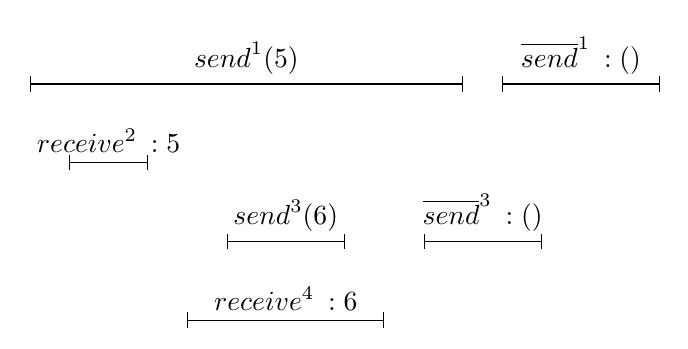
\begin{tikzpicture}
\draw[|-|] (0,0) -- node[above] {  $\sm{send}^1(5)$ } (5.5,0);
\draw[|-|] (6,0) -- node[above] { $\overline{\sm{send}}^1 \:: ()$ } (8,0);
\draw[|-|] (0.5,-1) -- node[above] { $\sm{receive}^2 \:: 5$} (1.5,-1) ;
\draw[|-|] (2.5,-2) -- node[above] {  $\sm{send}^3(6)$ } (4,-2);
\draw[|-|] (5,-2) -- node[above] { $\overline{\sm{send}}^3 \:: ()$ } (6.5,-2);
\draw[|-|] (2.0,-3)  -- node[above] { $\sm{receive}^4 \:: 6$} (4.5,-3);
\end{tikzpicture}
\scalaMid
\end{center}
%
Here, the invocations in the top two rows synchronise to transmit~5, and then
the invocations in the bottom two rows synchronise to transmit~6.  However,
the thread for the top row is slow to write its last three events into the
log.  The above history is not linearisable with respect to |TwoStepLinSpec|:
it is clear that $\sm{send}^1(5)$ and $\sm{receive}^2 \:: 5$ would need to be
linearised first; but this would require $\overline{\sm{send}}^1$ to be
linearised before $\sm{send}^3(6)$, which is inconsistent with the history.
Hence the approach would generate a false error.

Instead we use a technique that is robust against delays in logging.  We
assume that each thread has an identity in some range $\range 0
{\sm{NumThreads}}$.  We arrange for this identity to be included in the
$\call$ events written to the log for operations~|op|\s1 and
$\overline{\sm{op}}_1$, but otherwise threads act as above; in particular, for
each thread, calls to~|op|\s1 and $\overline{\sm{op}}_1$ alternate.

We then test whether the history is linearisable with respect to the
specification object below.  This object requires that corresponding
invocations of~|op|\s1 and~|op|\s2 are linearised consecutively: it encodes
the automaton on the right.  However, it allows
the corresponding $\overline{\sm{op}}_1$ to be linearised later (but before
the next operation invocation by the same thread).  It uses an array
|returns|, indexed by thread identities, to record values that should be
returned by a $\overline{\sm{op}}_1$ operation.
%
\begin{trivlist}
\item[]
\begin{minipage}{92mm}
\begin{scala}
type ThreadID = Int               // Thread identifiers
val NumThreads: ThreadID = ... // Number of threads
trait State
case class Zero extends State
case class One(t: ThreadID, x£\s1£: A£\s1£) extends State
\end{scala}
\end{minipage}
%%%%%
\hfill 
%
\begin{minipage}{37.8mm}
\begin{tikzpicture}[>= angle 60, xscale = 0.9, yscale = 0.44]
\draw (0,0) node[draw] (zero) {$\sm{Zero}$};
\draw[->] (zero) ++ (-1.5, 0) -- (zero);
%
\draw (0,-4) node[draw] (one) {$\sm{One}(\sm t, \sm{x}_1)$};
\draw[->] (zero) .. controls ++(0.3,-2) .. 
  node[right] {$\sm{op}_1(\sm t, \sm{x}_1)$} (one); 
%
%% \draw (2, -2) node[draw] (two) {$\sm{Two}(\sm{y}_1)$};
%% \draw[->] (one)  -- node[right] {$\sm{op}_2(\sm{x}_2)$} (two); 
\draw[->] (one) .. controls ++(-0.3,2) .. 
  node[left] {$\sm{op}_2(\sm x_2)$} (zero);
\end{tikzpicture}%
\end{minipage}%
%%%%%
\begin{scala}
object TwoStepDelayedLinSpec{
  private var state: State = Zero
  private val returns = new Array[Option[B£\s1£]](NumThreads)
  for(t <- 0 until NumThreads) returns(t) = None
  def op£\s1£(t: ThreadID, x£\s1£: A£\s1£): Unit = {
    require(state.isInstanceOf[Zero]); state = One(t, x£\s1£); ()
  }
  def op£\s2£(x£\s2£: A£\s2£): B£\s2£ = {
    require(state.isInstanceOf[One]); val One(t, x£\s1£) = state
    val (y£\s1£, y£\s2£) = SyncSpec.sync(x£\s1£, x£\s2£); returns(t) = Some(y£\s1£); state = Zero; y£\s2£
  }
  def £$\overline{\sm{op}}_1$£(t: ThreadID): B£\s1£ = {
    require(returns(t).isInstanceOf[Some]); val Some(y£\s1£) = returns(t)
    returns(t) = None; y£\s1£
  }
}
\end{scala}
\end{trivlist}

The following lemma identifies important properties of
|Two|\-|Step|\-|Delayed|\-|LinSpec|.  It follows immediately from the
definition.
%
\begin{lemma}
\label{lem:TwoStepDelayedLinSpec}
Within any legal history of |TwoStepDelayedLinSpec|, events $\op_1$ and
$\op_2$ alternate.  Let $\op_1^{i_1}(t,x_1) \:: ()$ and $\op_2^{i_2}(x_2) \::
y_2$ be a consecutive pair of such events.  Then |op|\s2 makes a call
$\sm{SyncSpec.sync}(x_1, x_2)$ obtaining result $(y_1,y_2)$.  Under the
assumptions about threads within the test, the next event for thread~$t$ will
be $\overline\op_1^{i_1}(t) \:: y_1$; and this will be later in the history
than $\op_2^{i_2}(x_2) \:: y_2$.  Further, the corresponding history of
events $\sm{sync}^{i_1,i_2}(x_1,x_2) \:: (y_1,y_2)$ is a legal history of
|SyncSpec|.

Conversely, each history with events ordered in this way will be a legal
history of |TwoStepDelayedLinSpec| if  the corresponding history
of events $\sm{sync}^{i_1,i_2}(x_1,x_2) \:: (y_1,y_2)$ is a legal history of
|SyncSpec|.
\end{lemma}


In order to argue for correctness, we need to distinguish between:
%
\begin{itemize}
\item the \emph{invocation history}, in terms of actual calls and returns of
  |op|\s1 and |op|\s2; and

\item the corresponding \emph{log history}, which might contain delays.
\end{itemize}
%
For clarity, we annotate events with ``$inv$'' or~``$log$''.  The invocation
history uses events of the form $\call^{inv}.\sm{op}_1^{i_1}(x_1)$,\,
$\return^{inv}.\sm{op}_1^{i_1} \:: y_1$,\,
$\call^{inv}.\sm{op}_2^{i_2}(x_2)$,\, and $\return^{inv}.\sm{op}_2^{i_2} \::
y_2$.  The log history uses events of the form
$\call^{log}.\sm{op}_1^{i_1}(t,x_1)$ (note the additional thread identity
parameter), $\return^{log}.\sm{op}_1^{i_1} \:: ()$ (note the unit return
value), $\call^{log}.\overline{\sm{op}}_1^{i_1}(t)$,\,
$\return^{log}.\overline{\sm{op}}_1^{i_1} \:: y_1$ (note the transferred
return value), $\call^{log}.\sm{op}_2^{i_2}(x_2)$, and
$\return^{log}.\sm{op}_2^{i_2} \:: y_2$

We can consider the interleaving of the invocation and log histories,
following real-time order.  In the interleaving, for |op|\s1 and |op|\s2,\,
$\call^{log}$ events will be earlier than the corresponding $\call^{inv}$
events; and $\return^{log}$ events will be later than the corresponding
$\return^{inv}$ events.  However, the two histories agree on the relative
order of the |op|\s1 and |op|\s2 events of each individual thread.

The proposition below shows that this testing method does not generate any false
errors. 
%
\begin{prop}
Suppose synchronisation object |SyncObj| is linearisable with respect
to~|SyncSpec|.  Then each complete log history~$h_l$ of |SyncObj| is
linearisable with respect to |TwoStepDelayedLinSpec|.
\end{prop}


\begin{proof}
Consider a complete log history~$h_l$ of~|SyncObj|, and a corresponding
invocation history~$h$; and consider their real-time interleaving.  By
assumption, there is a legal history~$h_s$ of |SyncSpec| such that $h$
and~$h_s$ are synchronisation compatible.  Thus $h_s$ may be interleaved with
the interleaving of~$h$ and~$h_l$, so that each $\sm{sync}$ event from~$h_s$
is between the corresponding $\call^{inv}$ and $\return^{inv}$ events
from~$h$, and hence also between the corresponding $\call^{log}$ and
$\return^{log}$ events from~$h_l$.

We build an interleaving of $h$, $h_l$ and a legal history $h_s'$ of
|Two|\-|Step|\-|Delayed|\-|LinSpec| from the interleaving of~$h$, $h_l$
and~$h_s$, as follows.
%
\begin{enumerate}
\item We replace each $\sm{sync}^{i_1,i_2}(x_1,x_2) \:: (y_1,y_2)$ by
  the two (consecutive) events $\sm{op}_1^{i_1}(t,x_1) \:: ()$ and
  $\sm{op}_2^{i_2}(x_2) \:: y_2$, where $t$ is the identity of the thread that
  makes the corresponding call of |op|\s1 in~$h_l$.  
  %% These are between the corresponding $\call$ and $\return$ events
  %% from~$h_l$ for each of $\sm{op}_1^{i_1}$ and $\sm{op}_2^{i_2}$, by
  %% construction.  Further, the relative order of all such events is the same
  %% as the order of the corresponding |sync| events, as required by
  %% |TwoStepDelayedLinSpec|; and the value of each~$y_2$ also agrees with
  %% |TwoStepDelayedLinSpec|.  Finally, the appropriate value~$y_1$ is written
  %% into $\sm{returns}(t)$.

\item We insert an event $\overline{\sm{op}}_1^{i_1}(t) \:: y_1$ between every
  $\call^{log}.\overline{\sm{op}}_1^{i_1}(t)$ and
  $\return^{log}.\overline{\sm{op}}_1^{i_1} \:: y_1$ (from~$h_l$), but not
  between any pair of $\sm{op}_1$ and $\sm{op}_2$ events from the previous
  stage.  \framebox{???}
  %% Because of the way logging is done, the value of~$y_1$ must match the value
  %% returned by the previous invocation of~|op|\s1 on the synchronisation object
  %% by thread~$t$; and this value much match the last value written into
  %% $\sm{returns}(t)$.  This again agrees with |TwoStepDelayedLinSpec|.
\end{enumerate}
%
Note that each inserted event is between the corresponding $\call^{log}$ and
$\return^{log}$ events, by construction.  Let $h_s'$ be these inserted events;
we show that $h_s'$ is a legal history of |Two|\-|Step|\-|Delayed|\-|LinSpec|.
\begin{itemize}
\item The events inserted in step~1 alternate between |op|\s1 and~|op|\s2, as
  required by |Two|\-|Step|\-|Delayed|\-|LinSpec|.  Further, they are in the
  same order, and have the same values for~$x_1$, $x_2$, $y_2$, $i_1$
  and~$i_2$ as the corresponding |sync| events from~$h_s$.  Hence each
  inserted |op|\s2 event has the return value~$y_2$ as required by
  |Two|\-|Step|\-|Delayed|\-|LinSpec|.  Further, the value for~$t$ matches
  that in the corresponding $\call^{log}.\sm{op}_1^{i_1}(t,x_1)$ event; so
  the value $y_1$ written into $\sm{returns}(t)$ (by~|op|\s2 in
  |Two|\-|Step|\-|Delayed|\-|LinSpec|) matches the value returned by the
  corresponding call to~|sync|.

\item For the events from step~2, because of the way logging is done, each
  value of~$y_1$ returned by $\overline{\sm{op}}_1$ must match the value
  returned by the previous invocation of~|op|\s1 on the synchronisation object
  by thread~$t$.  Since~$h$ is synchronisation linearisable, this $y_1$ must
  match the value returned by the corresponding call of~|sync|.  And this
  matches the last value written into $\sm{returns}(t)$ (by the previous
  item), as required by |Two|\-|Step|\-|Delayed|\-|LinSpec|.
\end{itemize}

%
%% Thus the events inserted form a legal history $h_s'$ of
%% |Two|\-|Step|\-|Delayed|\-|Lin|\-|Spec|, with each event between the
%% corresponding $\call$ and $\return$ events from~$h_l$.  
This demonstrates that
$h_l$ is linearisable with respect to |Two|\-|Step|\-|Delayed|\-|LinSpec|.
\end{proof}

%%%%%%%%%%

In theory, the delays in logging can mean that an invocation history that is
not synchronisation linearisable is transformed into a log history that is
linearisable with respect to |Two|\-|Step|\-|Delayed|\-|LinSpec| (although
this seems unlikely).  

We show that if the invocation history is not synchronisation linearisable
with respect to |SyncSpec|,
then there is a corresponding log history that is not linearisable with
respect to |Two|\-|Step|\-|Delayed|\-|LinSpec|.

\begin{prop}
\label{prop:TwoStepDelayedLinSpec-complete}
Let $h$ be a history of~|SyncObj| that is not synchronisation linearisable
with respect to |SyncObj|.  Then there is a corresponding log history~$h_l$
that is not linearisable with respect to |Two|\-|Step|\-|Delayed|\-|LinSpec|.
\end{prop}

%%%%%

\begin{figure}
\def\sep{1.5}
\begin{center}
\begin{tikzpicture}
\draw(0,0) node (h) {$h$:}; 
\draw(0,-\sep) node (h_l) {$h_l$:};
\draw(0,-\sep-\sep) node (h-s) {$h_s$:};
%% call.op_1
\draw (h)++(2,-0.2) node (call-inv-1) {\footnotesize $\call^i.\op_1$};
\draw[fill] (call-inv-1)++(0,0.4) circle (2pt); 
\draw (h_l)++(1.7,-0.2)node (call-log-1) {\footnotesize $\call^l.\op_1$};
\draw[fill] (call-log-1)++(0,0.4) circle (2pt); 
%% call.op_2 
\draw (call-inv-1)++(2,0) node (call-inv-2) {\footnotesize $\call^i.\op_2$};
\draw[fill] (call-inv-2)++(0,0.4) circle (2pt); 
\draw (call-log-1)++(2,0) node (call-log-2) {\footnotesize $\call^l.\op_2$};
\draw[fill] (call-log-2)++(0,0.4) circle (2pt);
%% return.op_1
\draw (call-inv-2)++(3,0) node (ret-inv-1) {\footnotesize $\return^i.\op_1$};
\draw[fill] (ret-inv-1)++(0,0.4) circle (2pt); 
%
\draw (call-log-2)++(3.6,0) node (ret-log-1) {\footnotesize $\return^l.\op_1$};
\draw[fill] (ret-log-1)++(0,0.4) circle (2pt); 
%
\draw (ret-log-1)++(1,0.8) node (call-log-1-bar) 
  {\footnotesize $\call^l.\overline\op_1$};
\draw[fill] (call-log-1-bar)++(0,-0.4) circle (2pt); 
%
\draw (ret-log-1)++(2,0) node (ret-log-1-bar) 
  {\footnotesize $\return^l.\overline\op_1$};
\draw[fill] (ret-log-1-bar)++(0,0.4) circle (2pt); 
%% return.op_2
\draw (ret-inv-1)++(4,0) node (ret-inv-2) {\footnotesize $\return^i.\op_2$};
\draw[fill] (ret-inv-2)++(0,0.4) circle (2pt); 
%
\draw (ret-inv-2)++(0.3,-\sep) node (ret-log-2)
   {\footnotesize $\return^l.\op_2$};
\draw[fill] (ret-log-2)++(0,0.4) circle (2pt); 
%% op_1
\draw (call-inv-1)++(1,-\sep-\sep) node (op-1) {\footnotesize $\op_1$};
\draw[fill] (op-1)++(0,0.4) circle (2pt); 
%% op_2
\draw (call-inv-2)++(1,-\sep-\sep) node (op-2) {\footnotesize $\op_2$};
\draw[fill] (op-2)++(0,0.4) circle (2pt); 
%% \overline{op}_1
\draw (call-log-1-bar)++(0.5,-\sep-0.8)  node (op-1-bar)
  {\footnotesize $\overline\op_1$};
\draw[fill] (op-1-bar)++(0,0.4) circle (2pt); 
\end{tikzpicture}
\end{center}
\caption{Representation of the construction in the proof of
  Proposition~\ref{prop:TwoStepDelayedLinSpec-complete}.  The interleaving of
  the histories is to be read from left to right.  The $\call$s of $\op_1$
  and~$\op_2$ might be in either order, as might their $\return$s.  The proof
  shows that both $\call$s precede both $\return$s.  We abbreviate ``$log$''
  and ``$inv$'' to~``$l$'' and~``$i$'', respectively.}
\label{fig:TwoStepDelayedLinSpec-complete}
\end{figure}

\begin{proof}
Let $h$ be as in the statement of the proposition.  We build a corresponding
log history~$h_l$, and interleave it with~$h$ as follows.  The construction is
illustrated in Figure~\ref{fig:TwoStepDelayedLinSpec-complete}.
%
\begin{itemize}
\item We add an event $\call^{log}.\op_1^{i_1}(t,x_1)$ immediately before
  each $\call^{inv}.\op_1^{i_1}(x_1)$, where $t$ is the identity of the
  thread making the call.

\item We add events $\return^{log}.\op_1^{i_1} \:: ()$,\,
  $\call^{log}.\overline{\op}_1^{i_1}(t)$, and
  $\return^{log}.\overline{\op}_1^{i_1} \:: y_1$ immediately after each
  $\return^{inv}.\op_1^{i_1} \:: y_1$, where again $t$ is the identity of the
  relevant thread.

\item We add an event $\call^{log}.\op_2^{i_2}(x_2)$ immediately before
  each $\call^{inv}.\op_2^{i_2}(x_2)$.

\item We add an event $\return^{log}.\op_2^{i_2} \:: y_2$ immediately after
  each  $\return^{inv}.\op_2^{i_2} \:: y_2$.

%% \item We add events $\call^{log}.\overline{\op}_1^{i_1}(t)$, and
%%   $\return^{log}.\overline{\op}_1^{i_1} \:: y_1$ immediately after the later
%%   of 
\end{itemize}
%
Let $h_l$ be these inserted events.  We need to show that $h_l$ is not
linearisable with respect to |Two|\-|Step|\-|Delayed|\-|LinSpec|.  We argue by
contradiction: we suppose that $h_l$ \emph{is} linearisable, and deduce that
$h$ is synchronisation linearisable with respect to |SyncSpec|.

So suppose $h_l$ is linearisable, and let $h_s$ be the corresponding legal
history of~|Two|\-|Step|\-|Delayed|\-|LinSpec|.  
%
Let $\op_1^{i_1}(t,x_1)\::y_1$ and $\op_2^{i_2}(x_2)\::y_2$ be two consecutive
events in~$h_s$.  Then:
%
\begin{enumerate}
\item In $h_l$, the event $\call^{log}.\op_1^{i_1}(t,x_1)$ is earlier than
  $\return^{log}.\op_2^{i_2} \:: y_2$ (to satisfy linearisation).  So in~$h$,
  the event $\call^{inv}.\op_1^{i_1}(t,x_1)$ is earlier than
  $\return^{inv}.\op_2^{i_2} \:: y_2$, by the way we have constructed~$h_l$.  

\item In $h_s$, the event $\op_2^{i_2}(x_2)\::y_2$ must be earlier than
  $\overline\op_1^{i_1}(t)\::y_1$ (by Lemma~\ref{lem:TwoStepDelayedLinSpec}).
  So in~$h_l$, the event $\call^{log}.\op_2^{i_2}(x_2)$ must be earlier than
  $\return^{log}.\overline{\op}_1^{i_1} \:: y_1$ (to satisfy linearisation).
  Hence, by the way we have constructed~$h_l$, the event
  %% $\call^{log}.\op_2^{i_2}(x_2)$ is also earlier than
  %% $\return^{log}.\op_1^{i_1} \:: ()$.  And hence, in~$h$, the event
  $\call^{inv}.\op_2^{i_2}(x_2)$ is earlier than $\return^{inv}.\op_1^{i_1}
  \:: y_1$.
  %, again by the way we have constructed~$h_l$.

%% \item In $h_s$, the event $\overline\op_1^{i_1}(t)\::y_1$ must be later than
%%   $\op_1^{i_1}(t,x_1)\::y_1$ and $\op_2^{i_2}(x_2)\::y_2$ (by
%%   Lemma~\ref{lem:TwoStepDelayedLinSpec}).  So in~$h_l$, the event
%%   $\return^{log}.\overline{\op}_1^{i_1} \:: y_1$ must be later than
%%   $\call^{log}.\op_2^{i_2}(x_2)$ (to satisfy linearisation).  Hence, by the
%%   way we have constructed~$h_l$, the event $\return^{log}.\op_1^{i_1} \:: ()$
%%   is also later than $\call^{log}.\op_2^{i_2}(x_2)$. And hence, in~$h$, the
%%   event $\return^{inv}.\op_1^{i_1} \:: y_1$ is later than
%%   $\call^{inv}.\op_2^{i_2}(x_2)$, again by the way we have constructed~$h_l$.
\end{enumerate}

%% It is clear that within~$h_s$, events $op_1$ and~$op_2$ alternate.  If
%% $op_1^{i_1}(x_1) \:: ()$ and $op_2^{i_2}(x_2) \:: y_2$ are consecutive such
%% events, then this represents a synchronisation of those invocations. 
%% The invocation of 
%% |Two|\-|Step|\-|Delayed|\-|LinSpec.op|\s2 calls $\sm{SyncSpec.sync}(x_1,x_2)$

%% Let $h_s'$ be the history of
%% corresponding calls to |SyncSpec.sync| from within
%% |Two|\-|Step|\-|Delayed|\-|LinSpec.op|\s2.  More precisely, each event
%% $\sm{sync}^{i_1,i_2}(x_1,x_2)\:: (y_1,y_2)$ corresponds to the call to
%% |SyncSpec.sync| within
%% |Two|\-|Step|\-|Delayed|\-|LinSpec.op|$_2^{i_2}(x_2)\::y_2$, where $x_1$ is
%% taken from |state|, so corresponds to the previous invocation of~$\op_1$, namely
%% $\op_1^{i_1}(x_1)$.  By the assumption, this must be a legal history
%% of~|SyncSpec|.

Let $h_s'$ be the legal history of |SyncSpec| corresponding to~$h_s$, implied
by Lemma~\ref{lem:TwoStepDelayedLinSpec}.  Given the interleaving of~$h_l$
and~$h_s$, and the interleaving of~$h_l$ and~$h_s$, we build an interleaving
of $h$ and~$h_s'$.  We insert each event $\sm{sync}^{i_1,i_2}(x_1,x_2)\::
(y_1,y_2)$ from~$h_s'$ after both $\call^{inv}.\op_1^{i_1}(t,x_1)$ and
$\call^{inv}.\op_2^{i_2}(x_2)$, but before both $\return^{inv}.\op_1^{i_1} \::
y_1$ and $\return^{inv}.\op_2^{i_2} \:: y_2$.  Note that this is possible,
because we have shown that $\call^{inv}.\op_1^{i_1}(t,x_1)$ is before
$\return^{inv}.\op_2^{i_2} \:: y_2$ (item~1 above), and
$\call^{inv}.\op_2^{i_2}(x_2)$ is before $\return^{inv}.\op_1^{i_1} \:: y_1$
(item~2 above).  Clearly this interleaving preserves the order of~$h_s'$.

Hence we have shown that $h$ is synchronisation compatible with~$h_s'$, and so
is linearisable with respect to |SyncSpec|, as required.

%% Within the interleaving of~$h_l$ and~$h_s$, each |sync| event is between the
%% corresponding $\call^{log}.\op_2$ and $\return^{log}.\op_2^{i_2}$ events.
%% Given this interleaving and the interleaving of~$h_l$ and~$h$, we can
%% construct a corresponding interleaving of all three histories, by ensuring
%% that each |sync| event is also between the corresponding $\call^{inv}.\op_2$
%% and $\return^{inv}.\op_2^{i_2}$ events.  


\end{proof}



%%%%%%%%%%%%%%%%%%%%%%%%%%%%%%%%%%%%%%%%%%%%%%%%%%%%%%%

\framebox{Previous version, not quite right}

However, if the delays are sufficiently small, then the
log history agrees with the invocation history on the |op|\s1 and~|op|\s2
events.  We show that in this case that log history is not linearisable.
%
\begin{lemma}
Consider an invocation history~$h$ that is not synchronisation linearisable
with respect to $SyncSpec$.  Let $h_l$ be a corresponding log~history that
agrees with~$h$ on |op|\s1 and~|op|\s2 events.  Then $h_l$ is not linearisable
with respect to |Two|\-|Step|\-|Delayed|\-|LinSpec|.
\end{lemma}

%%%%%

\begin{proof}
We prove the contrapositive: we suppose that $h_l$ is linearisable with
respect to |Two|\-|Step|\-|Delayed|\-|LinSpec|, and show that $h$ is
synchronisation linearisable with respect to |SyncSpec|. 

From the assumption that $h_l$ is linearisable, there is a legal history~$h_s$
of |Two|\-|Step|\-|Delayed|\-|LinSpec| such that $h_l$ and~$h_s$ are
compatible.  Consider the interleaving of $h_l$ and~$h_s$.  Since $h_l$
and~$h$ agree on the |op|\s1 and~|op|\s2 events, we can build a corresponding
interleaving of $h$ and~$h_s$: so each $\sm{op}_1^{i_1}(t,x_1)\::()$ event is
between events $\call^{inv}.\sm{op}_1^{i_1}(x_1)$ and
$\return^{inv}.\sm{op}_1^{i_1} \:: y_1$, where $t$ is the identity of the
thread making the call; and each $\sm{op}_2^{i_2}(x_2)\::y_2$ event is
between events $\call^{inv}.\sm{op}_2^{i_2}(x_2)$ and
$\return^{inv}.\sm{op}_2^{i_2} \:: y_2$.   

In |Two|\-|Step|\-|Delayed|\-|LinSpec|, each invocation of $\op_2(x_2)$ calls
$\sm{SyncSpec.sync}(x_1, x_2)$, obtaining result $(y_1, y_2)$, and
returns~$y_2$.  Here~$x_1$ is taken from |state|, and matches the parameter
of the previous  $\sm{op}_1^{i_1}(t,x_1)\::()$ event in~$h_s$.

%
We build a history $h_s'$ of~|SyncSpec| by replacing each event
$\sm{op}_2^{i_2}(x_2)\::y_2$ from~$h_s$ by $\sm{sync}^{i_1,i_2}(x_1, x_2) \::
(y_1,y_2)$ for the corresponding~$x_1$ and~$i_1$.  This is a legal history
of~|SyncSpec| by construction.  Likewise, each such event is between the
corresponding events $\call^{inv}.\sm{op}_2^{i_2}(x_2)$ and
$\return^{inv}.\sm{op}_2^{i_2} \:: y_2$, by construction.  

\end{proof}


%%%%%%%%%%%%%%%%%%%%%%%%%%%%%%%%%%%%%%%%%%%%%%%%%%%%%%% 

\subsection{Case with state}

Suppose the specification object has non-trivial state. 

I think it will be more efficient to give a more direct implementation.
Define a configuration to be: (1)~a point in the log reached so far; (2)~the
set of pending operation invocations that have not synchronised; (3)~the set
of pending operation invocations that have synchronised (but not returned);
and (4)~the state of the sequential synchronisation object.  In any
configuration, can: synchronise a pair of pending operations (and update the
synchronisation object); advance in the log if the next event is a return that
is not pending; or advance in the log if the next event is a call.  Then
perform DFS.

Partial order reduction: a synchronisation point must follow either the
call of one of the concurrent operations, or another synchronisation
point.  Any synchronisation history can be transformed into this form, by
moving synchronisation points earlier, but not before any of the corresponding
call events, and preserving the order of synchronisations.  This means that
after advancing past the call of an invocation, we may synchronise that
invocation, and then an arbitrary sequence of other invocations. 

Alternatively, a synchronisation point must precede either the return of one
of the concurrent operations, or another synchronisation point.  This is more
like the JIT technique in the linearisability testing paper.  This means that
before advancing in the log to the return of an invocation that has not
synchronised, we synchronise some invocations, ending with the one in
question.  And we only synchronise in these circumstances. 

My intuition is that the former is more efficient: in the latter, we might
investigate synchronising other invocations even though the returning
operation can't be synchronised with any invocation.  

%%%%%

\subsubsection*{Complexity}

Consider the problem of testing whether a given concurrent history has
synchronisations consistent with a given sequential specification object. 

We make use of a result from~\cite{???} concerning the complexity of the
corresponding problem for linearizability.  Let |Variable| be a
linearizability specification object corresponding to a variable with |get|
and |set| operations.  Then the problem of deciding whether a given concurrent
history is linearisable with respect to |Varaiable| is NP-complete.

Let |ConcVariable| be a concurrent object that represents a variable.  

We consider concurrent synchronisation histories on an object with the
following signature.   
\begin{scala}
object VariableSync{
  def op£\s1£(op: String, x: Int): Int
  def op£\s2£(u: Unit): Unit
} 
\end{scala}
%
The intention is that |op|\s1|("get", x)| acts like |get(x)|, and
|op|\s1|("set", x)| acts like |set(x)| (but returns -1).  The |op|\s2
invocations do nothing except synchronise.  This can be captured formally by
the following synchronisation specification object.

\begin{scala}
object VariableSyncSpec{
  private var state = 0
  def sync((op, x): (String, Int), u: Unit): (Int, Unit) = 
    if(op == "get") (state, ()) else{ state = x; (-1, ()) }
}
\end{scala}


Let |ConcVariable| be a concurrent object that represents a variable.  Given a
concurrent history~$h$ of |ConcVariable|, we build a concurrent history~$h'$
of |VaraibleSync| as follows.  We replace every call or return of |get(x)| by
(respectively) a call or return of |op|\s1|("get", x)|; and we do similarly
with |set|s.  If there are $k$ calls of |get| or |set| in total, we prepend
$k$ calls of |op|\s2, and append $k$ corresponding returns (in any order).
Then it is clear that $h$ is linearisable with respect to |Variable| if and
only if $h'$ is linearisable with respect to |VariableSyncSpec|.

%%%%%%%%%%%%%%%%%%%%%%%%%%%%%%%%%%%%%%%%%%%%%%%%%%%%%%%%%%%%

\subsection{Stateless case}

In the stateless case, a completely different algorithm is possible.  Define
two invocations to be compatible if they could be synchronised, i.e.~they
overlap and the return values agree with those for the specification object.
For $n$ invocations of each operation (so a history of length~$4n$), this can
be calculated in $O(n^2)$.  Then find if there is a total matching in the
corresponding bipartite graph, using the Ford-Fulkerson method, which is
$O(n^2)$.
